\section*{Results}

In Figure 4, we showcase our first successful keep-alive connection. Here, two threads each handle a series of requests over a single connection, rather than multiple separate connections. In Figure 5, we present our first running CGI script, which outputs dynamic data, such as the user's IP address, that cannot be generated by a static file.
% And a simple CGI Script where we display the environment variables REMOTE\_HOST and REMOTE\_ADDR. 

\begin{figure}[h]
    \centering
    \begin{minipage}{0.55\textwidth}
        \centering
        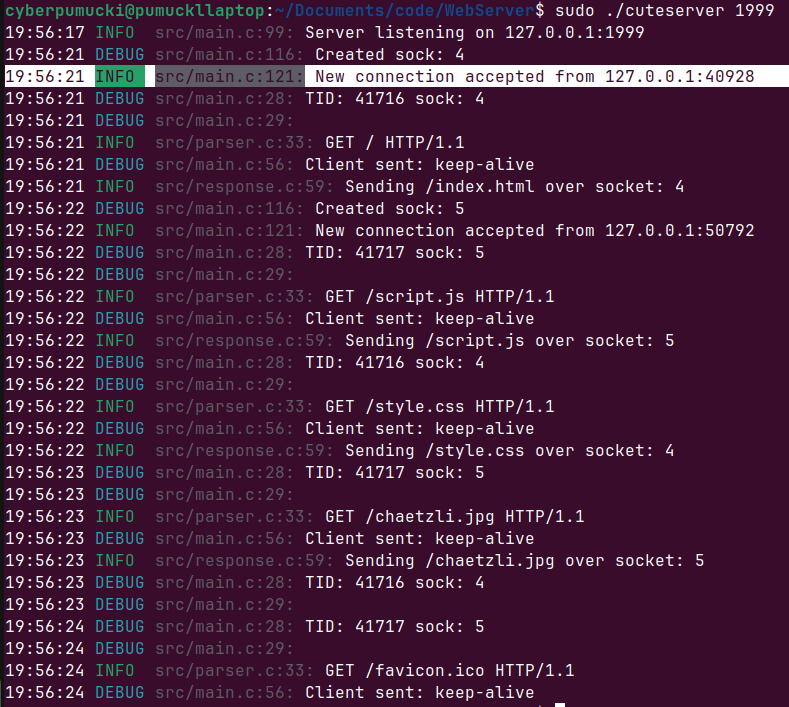
\includegraphics[width=\textwidth]{figures/keep-alive.png}
        \caption{Keep-Alive: Multiple Requests handled over one Connection}
    \end{minipage}
    \hfill
    \begin{minipage}{0.35\textwidth}
        \centering
        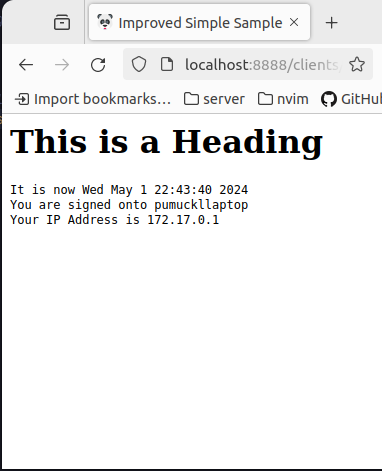
\includegraphics[width=\textwidth]{figures/cgi.png}
        \caption{First simple CGI Script with Environment Variables}
    \end{minipage}
\end{figure}
\vspace{-15pt}
\subsection*{Performance Testing}
We wanted to test the influence of the number of worker threads on the performance of our application. For this we used \textbf{Locust} \footnote{https://locust.io/} to tests POST and GET requests to our application, as well as static file requests. \\

\textbf{Static File Tests}: 
We conducted these tests using the following Locust Configuration: 500 virtual users, ramping up at 50 users/second, for a runtime of 60 seconds.Requests were made to a static file hosted on a home server with 4 cores, and multithreading was managed by OpenMP.
The graphs for 2 versus 3 worker threads exhibit similar trends, so the application runs relatively stable. The graph shows an initial peak in response time, followed by a gradual decline and stabilization at lower values. We can only explain this result by assuming that the responses are being cached somewhere.
The number of requests is similar, but the average response time with 2 threads is 239.07ms, while with 3 threads, it is 154.19ms—a reduction of about 85ms. This indicates that multithreading reduces the response time per request.

\begin{figure}[h]
    \centering
    \begin{minipage}{0.45\textwidth}
        \centering
        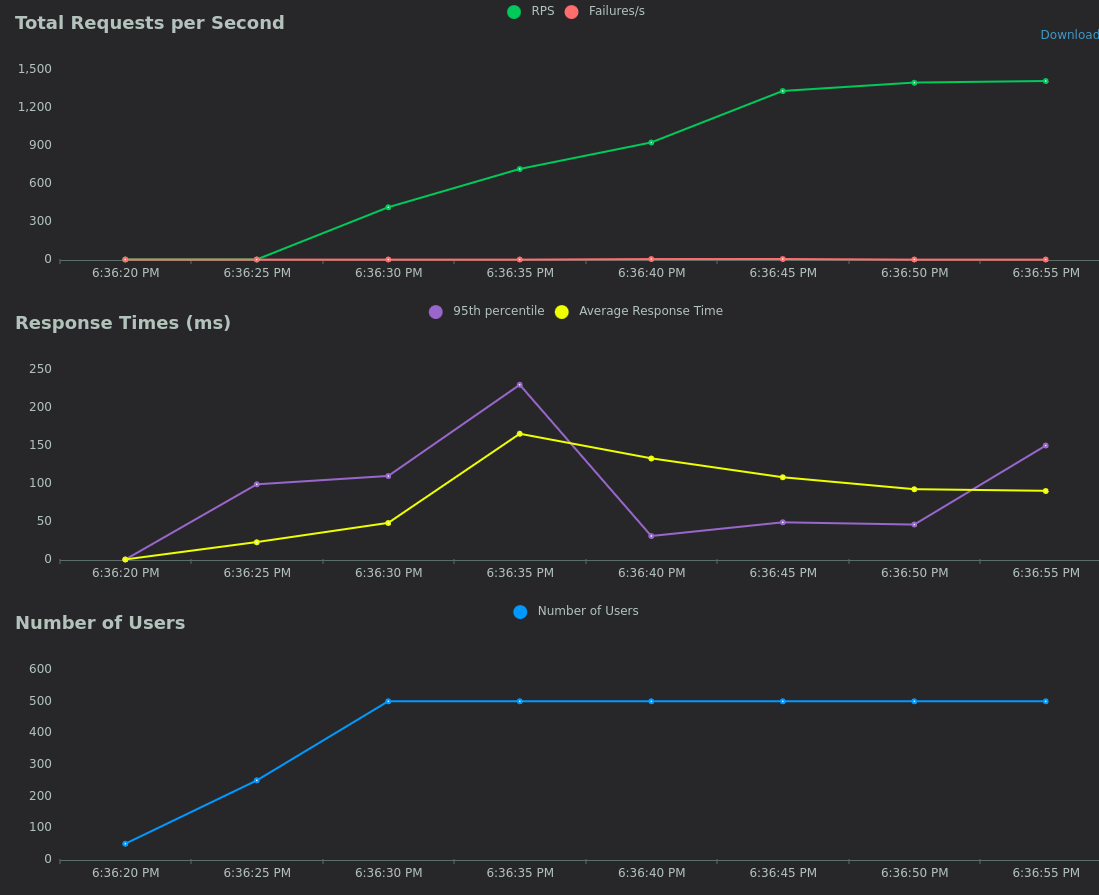
\includegraphics[width=\textwidth]{figures/2threads.png}
        % 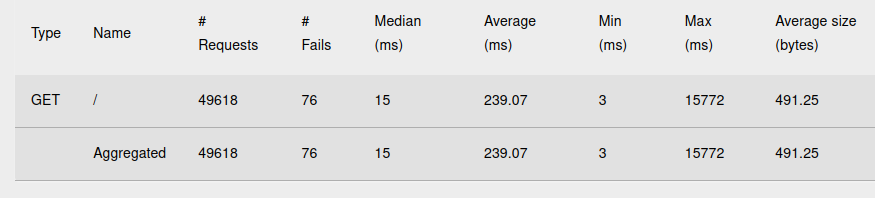
\includegraphics[width=\textwidth]{figures/2_threads_chart.png}
        \caption{Results with 2 Worker Threads}
    \end{minipage}
    \hfill
    \begin{minipage}{0.45\textwidth}
        \centering
        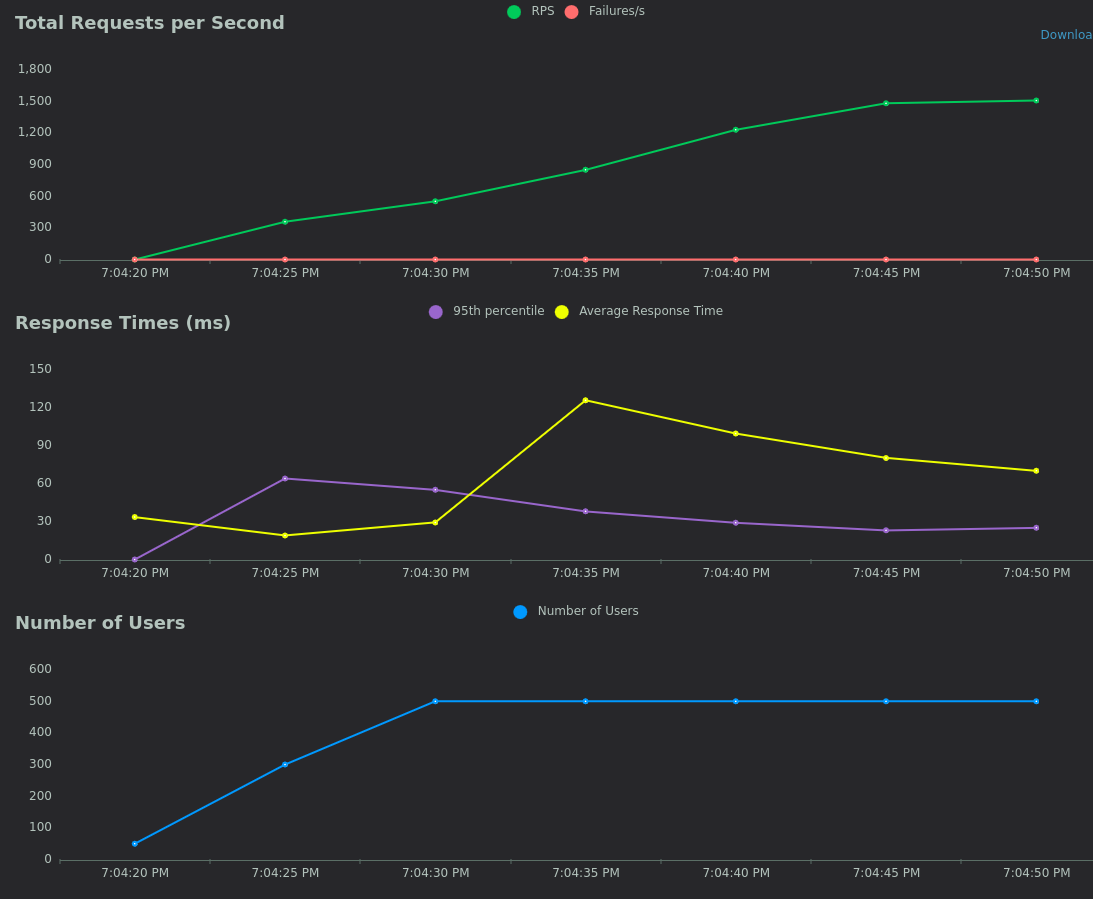
\includegraphics[width=\textwidth]{figures/3threads.png}
        % 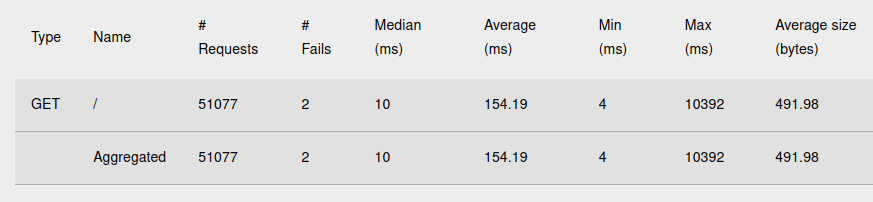
\includegraphics[width=\textwidth]{figures/3_threads_chart.png}
        \caption{Results with 3 Worker Threads}
    \end{minipage}
\end{figure}


